%----------------------------------------------------------------------------
\chapter{Változók használatának vizsgálata}
\label{chap:varUsage}
%----------------------------------------------------------------------------
%
% Bevezető
%
Az EMF-IncQuery lekérdezőnyelve -- más program- és leírónyelvekhez hasonlóan -- több olyan problémának is áldozatul esik, melyek statikus analízis segítségével hamar felismerhetőek, és a fejlesztők az analízis eredményét jó hatékonysággal használhatják fel az azonosított problémák orvoslására.
Az egyik leggyakoribb ilyen kellemetlenség a változók nevének (azonosítójának) nem konzisztens használata -- magyarul elírása -- a kód különböző pontjain, mellyel szinte minden informatikus találkozott már valamilyen formában.
A lekérdezőnyelv sajátossága miatt -- miszerint a lokális változókat nem szükséges előre deklarálni, mivel ezt a környezet impliciten, azok első előfordulásakor megteszi a fejlesztő helyett -- a kódban található kifejezések ilyen gépelési hibák elfordulása mellett is mindig szintaktikailag helyesek maradnak.
Így az ez által okozott hibák felderítéséhez a szemantikának, a kód jelentésének vizsgálatára van szükség, különben a hibára csak a lekérdezések futtatása után derülhet fény, melyre a rossz találati eredmények utalnak, és a hiba valódi oka még ekkor sem mindig egyértelmű.

%----------------------------------------------------------------------------
\section{Tervezés}

Az ilyen típusú ellenőrzés messze nem példa nélküli, más programozási nyelveknél és fejlesztőkörnyezeteknél gyakran találkozhatunk vele \emph{``nem használt változó detektálás''} néven.
Ám mivel az EMF-IncQuery lekérdezőnyelvében a változó fogalma kissé eltér a legtöbb nyelvben megszokottól, más környezetek megoldásai nem alkalmazhatóak egy az egyben.
Mint azt a \ref{chap:techPrim}. fejezetben már leírtam, a lekérdezőnyelv mintái esetében kétféle változóról beszélhetünk:
\begin{itemize}
    \item a \emph{paraméterváltozók}, melyek egy minta paraméterei, illetve
    \item a \emph{lokális változók}, amelyek egy mintának egy bizonyos törzsén belül fordulnak csak elő.
\end{itemize}
Ezek a változók leginkább az elsőrendű logika, illetve az ezen alapuló program- és lekérdezőnyelvek (pl. Prolog \cite{Colmerauer93thebirth}, Datalog \cite{Ceri:1989:YAW:627272.627357}) változóihoz hasonlíthatóak, így nem meglepő hogy beszélhetünk egy változó kvantifikáltságáról \cite{Huth:2004:LCS:975331}.

Mind a paraméterváltozók, mind a lokális változók lehetnek -- elméletben -- egzisztenciálisan vagy univerzálisan kvantifikálva, ám nem minden kombináció használható minden helyzetben, és a kétféle változókra valamelyest eltérő szabályok vonatkoznak.
A paraméterváltozóknak mindenképp felsorolható értékhalmazzal kell rendelkezniük, hiszen a mintaillesztőnek végső soron elő kell állítania az illeszkedések halmazát, ezen változókhoz is értéket rendelve.
Emiatt ezeknek a változóknak szükségszerűen egzisztenciálisan kvantifikáltaknak ($\exists x$) kell lenniük.
Univerzálisan kvantifikáltak ($\forall x$) nem lehetnek, hiszen akkor az összes elképzelhető modellentitásra kellene megvizsgálnunk a minta illeszkedését, ami pedig egy megoldhatatlan probléma, mivel ezek halmaza végtelen elemű, ugyanis az EMF-IncQuery szemantikája szerint az attribútumértékek is megköthetőek változóba.
Ugyanez a logika igaz általánosságban a lokális változókra is, egy kivétellel: a lokális változó lehet univerzálisan kvantifikálva, ha pontosan egy, \emph{negatívan alkalmazott} kényszerben szerepel.
A negatívan alkalmazott kényszerek negatív egzisztenciális kvantifikációt ($\neg\exists x$) jelentenek, ami az alábbi egyenlet alapján univerzális kvantifikációvá alakítható:
\begin{equation} \label{eq:negexiststoforall}
\neg\exists x\, P(x) \equiv \forall x\, \neg P(x)
\end{equation}
Ilyenkor a lokális változó ugyan univerzálisan van kvantifikálva, de az értékkészletét felsorolni sosem kell, hiszen egy negatív kényszerben szerepel, ami azt jelenti, hogy a kényszernek nem kell, sőt, nem is szabad teljesülnie.

Létezik még az úgynevezett \emph{read-only} kategóriába sorolható hivatkozás.
Ez olyan kifejezésekben fordul elő, ahol a kifejezés értéke alapján nem határozhatóak meg a kiértékelése során számba vett entitások.
Emiatt az ilyen kifejezéseket is univerzálisan kvantifikálónak tekinthetjük, mivel egzisztenciálisan nem kvantifikálják paramétereiket.
Ilyen kifejezések az ellenőrzés kényszerben lévő Java kifejezés és az aggregátor kifejezések.
%\todo{Az attribútumvizsgálat, pl. check (A<B) szerintem tök szemléletes további példa lenne itt, és jól elmagyarázható, hogy miért read only ez a változóhivatkozás}

A fent leírtakból következik, hogy \emph{egy paraméterváltozóra a minta minden törzsében lennie kell legalább egy egzisztenciálisan kvantifikáló hivatkozásnak}.
Egy lokális változó hivatkozásai két konstellációban fordulhatnak elő:
\begin{itemize}
    \item vagy egyetlen egy hivatkozás egy univerzálisan kvantifikáló, de negatívan alkalmazott kényszerben,
    \item vagy egy egzisztenciálisan kvantifikáló hivatkozás, illetve ezen kívül akárhány más hivatkozás
\end{itemize}
Az első esetben érdemes egyszer használatos változót alkalmaznunk, ami jelzi, hogy a változót máshol már nem szabad hivatkozni.
A második esetben szintén ajánlott egyszer használatos változót használnunk, \emph{ha} csak pontosan egy, egzisztenciálisan kvantifikáló hivatkozásunk van a változóra.
Ezzel jelezhetjük, hogy a változóra szándékosan nem hivatkozunk máshol.
Ellenkező esetben felmerülhet a kérdés, hogy a hivatkozás tényleg egy olyan új változót vezet be\footnote{Emlékeztető: a lokális változók első hivatkozásuknál impliciten deklarálódnak}, amelyre csak egyszer szerettünk volna hivatkozni, vagy a hivatkozás egy másik változóra irányult volna, de a változó nevét elgépeltük.

Tehát a változó típusától és a rá történő hivatkozások minőségétől és mennyiségétől függ, hogy a felhasználó milyen figyelmeztetést vagy hibaüzenetet kap, melyet részletesen az \ref{tab:warningsErrors}. táblázat mutat.
%
\tabulinesep=4pt
\begin{longtabu} to \textwidth{|X[1.5,c,m]|X[1,c,m]|X[1,c,m]|X[1,c,m]|X[3,c,m]|}
\caption{Figyelmeztetések és hibaüzenetek\label{tab:warningsErrors}} \\
\hline
& \multicolumn{3}{c|}{Változóhivatkozások a törzsben} & \\ \cline{2-4}
Változó & Pozitív & Negatív & Read-only & Üzenet típusa \\
\tabucline[1.5pt]{-}
\endfirsthead
\caption{Figyelmeztetések és hibaüzenetek (folyt.)} \\
\hline
& \multicolumn{3}{c|}{Változóhivatkozások a törzsben} & \\ \cline{2-4}
Változó & Pozitív & Negatív & Read-only & Üzenet típusa \\
\tabucline[1.5pt]{-}
\endhead
\multicolumn{5}{r}{\textit{a táblázat folytatódik a következő oldalon\ldots}} \\
\endfoot
\endlastfoot
Paraméter & 0    & 0    & 0    & Hiba: nincs hivatkozás a változóra \\
\hline
Lokális   & 1    & 0    & 0    & Figyelmeztetés: egyszer használt változó \\
\hline
Paraméter & 0    & 1    & 0    & Hiba: univerzálisan kvantifikált paraméterváltozó \\
\hline
Lokális   & 0    & 0    & 1    & Hiba: univerzálisan kvantifikált lokális változó \\
\hline
Paraméter & 0    & 0    & 1    & Hiba: univerzálisan kvantifikált paraméterváltozó \\
\hline
Lokális   & 0    & 0    & több & Hiba: univerzálisan kvantifikált lokális változó \\
\hline
Paraméter & 0    & 0    & több & Hiba: univerzálisan kvantifikált paraméterváltozó \\
\hline
Lokális   & 0    & 1    & 1    & Hiba: univerzálisan kvantifikált lokális változó \\
\hline
Paraméter & 0    & 1    & 1    & Hiba: univerzálisan kvantifikált paraméterváltozó \\
\hline
Lokális   & 0    & 1    & több & Hiba: univerzálisan kvantifikált lokális változó \\
\hline
Paraméter & 0    & 1    & több & Hiba: univerzálisan kvantifikált paraméterváltozó \\
\hline
Lokális   & 0    & több & 0    & Hiba: univerzálisan kvantifikált lokális változó \\
\hline
Paraméter & 0    & több & 0    & Hiba: univerzálisan kvantifikált paraméterváltozó \\
\hline
Lokális   & 0    & több & 1    & Hiba: univerzálisan kvantifikált lokális változó \\
\hline
Paraméter & 0    & több & 1    & Hiba: univerzálisan kvantifikált paraméterváltozó \\
\hline
Lokális   & 0    & több & több & Hiba: univerzálisan kvantifikált lokális változó \\
\hline
Paraméter & 0    & több & több & Hiba: univerzálisan kvantifikált paraméterváltozó \\
\hline
\end{longtabu}

%----------------------------------------------------------------------------

\section{Ellenőrzések}

Most lássunk néhány gyakorlati példát az eddig leírtakra.

\subsection{Hivatkozás nélküli paraméterváltozó}

Előfordulhat, hogy egy paraméterváltozóra nincs hivatkozás a minta egyik törzsében.

\begin{lstlisting}
package karate.incquery

import "http://karate/1.0"

pattern exampleQuery(student) = e_{
    Student(other);
    Student.name(other, "Daniel LaRusso");
}_
\end{lstlisting}
%
Ez hiba, mivel a változó így univerzálisan kvantifikálódik, ezért a mintaillesztő az adott törzs kiértékelésekor nem tud értéket rendelni a paraméterhez.

\subsection{Pozitív hivatkozás nélküli paraméterváltozó}

Előfordulhat az is, hogy van ugyan hivatkozás a paraméterváltozóra, de azok egyike sem (pozitív) egzisztenciális kvantifikáció.

\begin{lstlisting}
package karate.incquery

import "http://karate/1.0"

pattern notDaniel(student) = e_{
    neg Student.name(student, "Daniel LaRusso");
}_
\end{lstlisting}
%
% Megtévesztő, mert azt hinnénk hogy helyes, pedig nem.
%
vagy
%
\begin{lstlisting}
package karate.incquery

import "http://karate/1.0"
import "http://www.eclipse.org/emf/2002/Ecore"

pattern allStudents(student) = {
    Student(student);
}

pattern exampleQuery(student) = e_{
    EInt(n);
    n == count find allStudents(student);
}_
\end{lstlisting}
%
% Itt \texttt{s} csak bemeneti irányú (read-only) változó.
%
A probléma megegyezik az előző ellenőrzésnél látottal: a változó univerzálisan kvantifikált, a mintaillesztő nem tudja a változó értékhalmazát meghatározni.

\subsection{Lokális változó egyszeri hivatkozással}

Ha egy lokális -- de nem egyszer használatos -- változó csak egyszer kerül megemlítésre a kódban, akkor változók közti kapcsolat leírására nem szolgálhat -- ugyanis ahhoz legalább kétszer kellene szerepelnie.
Az ilyen helyzet elgépelésre vagy más hiányosságra utal.

\begin{lstlisting}
package karate.incquery

import "http://karate/1.0"

pattern isStudentOfMiyagi(student) = {
    Student(student);
    Student.master.name(w_studnet_, "Kesuke Miyagi");
}
\end{lstlisting}
,
\begin{lstlisting}
package karate.incquery

import "http://karate/1.0"

pattern studentsWhoHaveMaster(student) = {
    Student(student);
    Master(w_master_);
    // ez a sor maradhatott le: Student.master(student, master);
}
\end{lstlisting}
, illetve
%
\begin{lstlisting}
package karate.incquery

import "http://karate/1.0"

pattern allStudents(student) = {
    Student(student);
}

pattern numberOfStudents(n) = {
    EInt(n);
    n == count find allStudents(w_student_);
}
\end{lstlisting}

A fenti három esetben nem mondhatjuk egyértelműen, hogy hibázott a felhasználó, de szeretnénk felhívni a figyelmét a hibalehetőségre, ezért itt figyelmeztetést (warning) használunk.
Ha valóban csak helykitöltésre használjuk a változót -- mert nem érdekel minket például egy sok paraméteres minta néhány paramétere --, akkor használjunk anonim vagy egyszer használatos változót, hogy jelezzük szándékunkat és figyelmen kívül hagyjuk az ellenőrzést.

\subsection{Pozitív hivatkozás nélküli lokális változó}

Az egynél többször hivatkozott lokális változóknak, a paraméterváltozókhoz hasonlóan, szintén szükséges, hogy szerepeljenek legalább egy pozitív egzisztenciálisan kvantifikáló kifejezésben.
%
\begin{lstlisting}
package karate.incquery

import "http://karate/1.0"

pattern isShortName(name) = {
    Karateka.name(_, name);
    check(name.length < 10);
}

pattern longNamesExistThatAreNotMiyagi() = {
    neg find isShortName(e_name_);
    name != "Kesuke Miyagi";
}
\end{lstlisting}
%
Pozitív egzisztenciális kvantifikáció híján univerzálisan kvantifikálódik a \texttt{student} változó, így a mintaillesztő nem képes meghatározni értékhalmazát.

%----------------------------------------------------------------------------

\section{Implementáció}

A megtervezett ellenőrzés megvalósítását Java alapú Xtext validátor segítségével oldottam meg.
A validátor függvény egyetlen paramétere egy minta törzsét reprezentáló objektum, amelyen az ellenőrzést végezni fogja.
Az Xtext keretrendszer ezt a függvényt a validációs folyamat részeként minden ellenőrzésre kerülő minta összes törzsére egyenként meghívja.
A függvény egy mintatörzsben először megkeresi és minőségi csoportonként leszámlálja a törzsben és a törzshöz tartozó minta fejében található változóhivatkozásokat, majd az így felépített adatbázist bejárva megvizsgálja az egyes változókat a rájuk érvényes szabályok szerint, és ha szükséges, figyelmeztetést vagy hibaüzenetet emittál.
Az implementáció nem tér ki a tetszőleges Java kódot tartalmazó ellenőrzés kényszer és \texttt{eval} aggregátor kifejezés vizsgálatára, mivel az túlmutat a dolgozat keretein.

Az ellenőrzést működés közben a \ref{fig:unusedLive}. ábra mutatja.
\begin{figure}[!t]
\centering
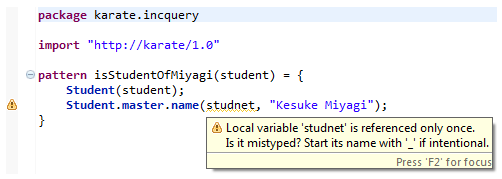
\includegraphics[width=0.90\textwidth]{figures/unused-variable-detection-warning.png}
\caption{Az elkészült ellenőrzés futás közben}
\label{fig:unusedLive}
\end{figure}

A validátor működésének teszteléséhez JUnit teszteket is készítettem, illetve frissítettem a már meglévő unitteszteket. Ezek segítenek a nyelv jövőbeni változása, bővítése miatt szükséges módosítások során az esetleges hibák megtalálásában (regresszió tesztelés), illetve valamilyen szinten bemutatják, biztosítják az elkészült ellenőrzések hatásosságát is.
